\vspace*{-5mm}
\mysection{Overall Description}

\mysubsection{Product Perspective}
The system, for achieving its goals, it will be related with three kind of external components :
\begin{itemize}
	\setlength{\leftskip}{0.5cm}
	\item Root providers (Google maps)
	\item Local transport services
	\item Outdoor transport services
\end{itemize}
To localize the means and the user’s positions and to retrieve the directions, we will use in our system Google maps API. The system will format the data received in a standardized manner and show them to the user according to his preferences.\par
Our system will contain all the references to the local and outdoor transport services, which APIs will be known in order to retrieve the requested information about the tickets’ prices. 
Once the user has chosen the ticket, he will be addressed to the service’s website to complete the purchase.\par
At first the system will advise about the best local transport tickets only in the towns of Milano, Torino and Rome; for the other towns, the system will give the user the possibility to access to the local transport websites.
Regarding the outdoor travels, it will be possible to buy tickets only with a restricted group of transport services such as Trenitalia and Alitalia.
\begin{figure}[H]
	\centering
	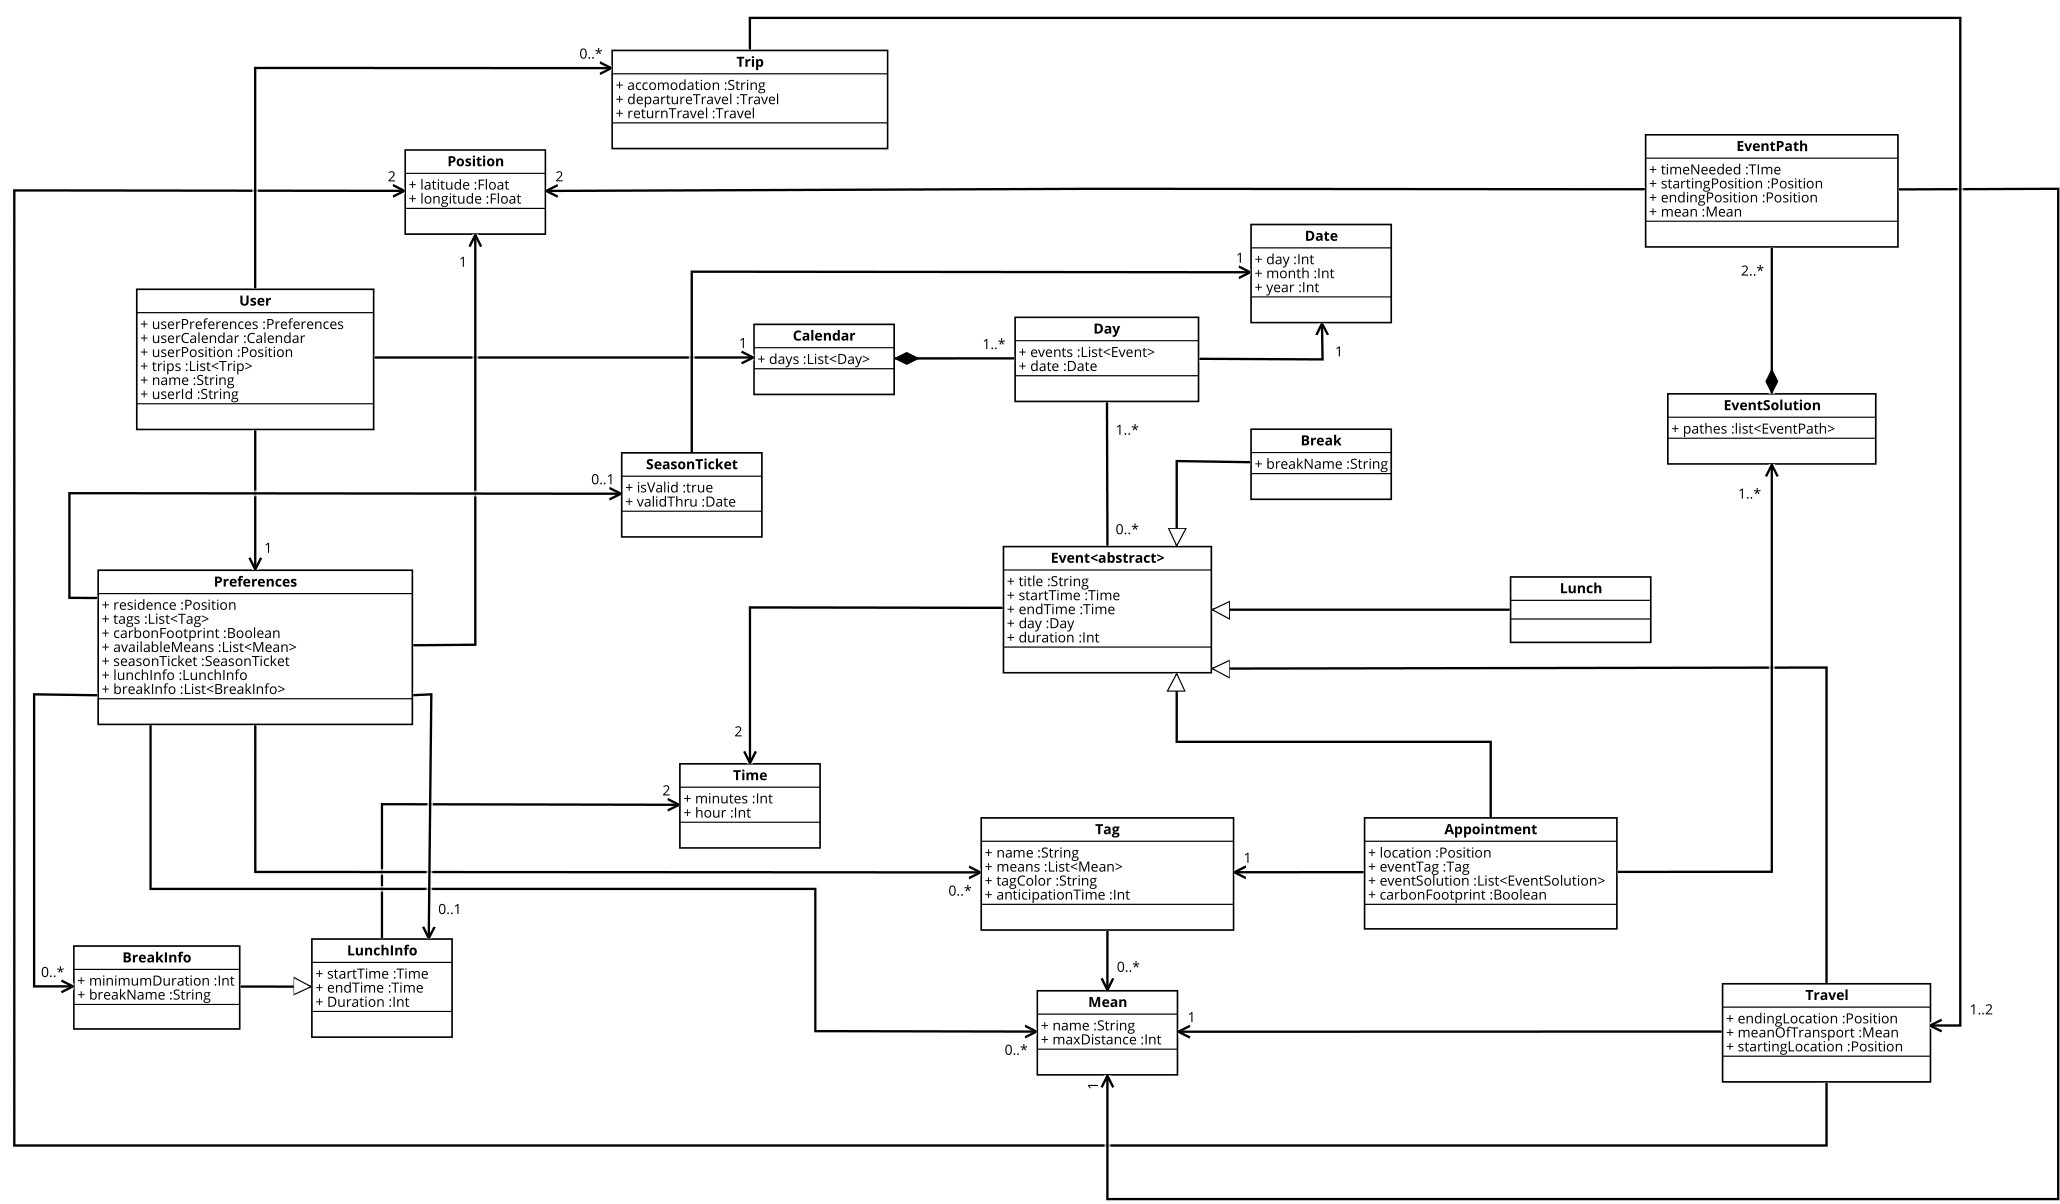
\includegraphics[scale=0.25]{Images/Class_Diagram}
	\caption{Class Diagram}
\end{figure}

\mysubsection{Product Functions}
In order to provide a clear vision of the system’s aims that will be implemented, we are going to show some use cases diagram representing the system’s features. A description of the main ones will be provided.
\begin{figure}[H]
	\centering
	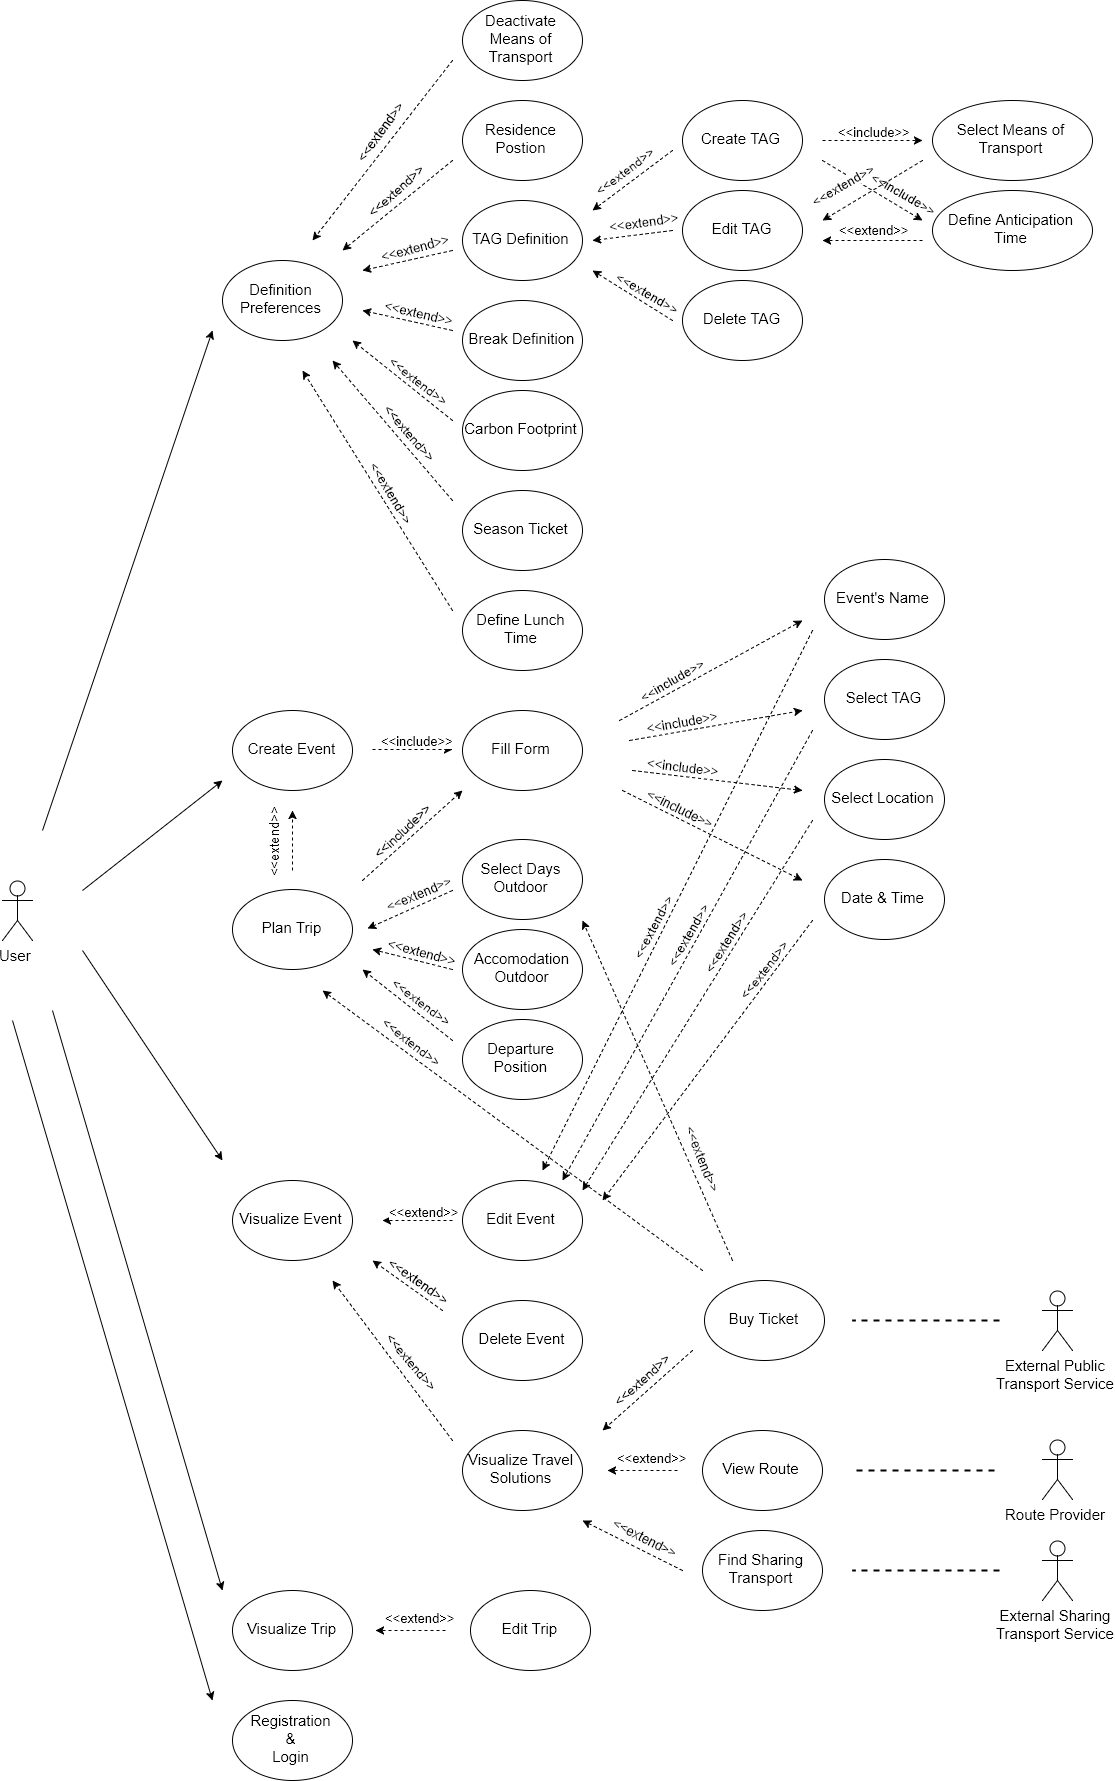
\includegraphics[scale=0.25]{Images/Use_Case/General_Use_Case}
	\caption{General Use Case}
\end{figure}

\mysubsubsection{Registration \& Login}
The system will let the user to sign up, inserting the e-mail and password for creating his personal profile and he will be able to sign-in every time he wants.

\mysubsubsection{Set Preferences}
\begin{figure}[H]
	\centering
	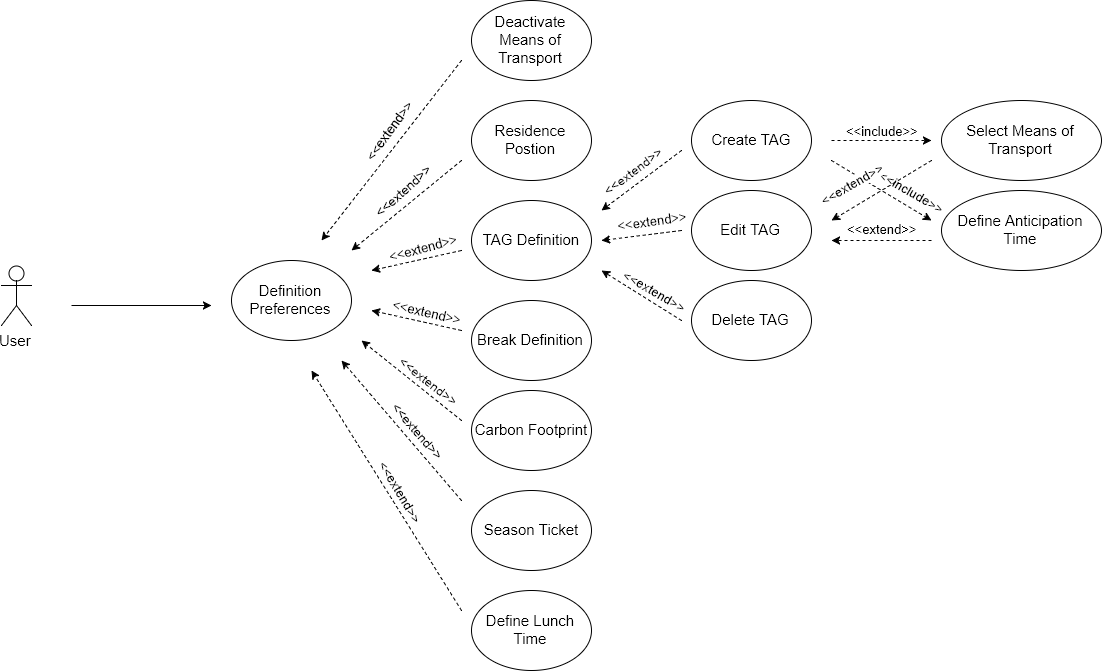
\includegraphics[scale=0.25]{Images/Use_Case/Set_Preferences}
	\caption{Set Preferences Use Case}
\end{figure}
The user will be able to set many preferences to customize his profile. 
He will be able to :
\begin{itemize}
	\setlength{\leftskip}{1cm}
	\item insert his season ticket and receive warnings to remind him the expiry date.
	\item set his home address that will allow the system to compute the routes for reaching the first event of the day using it as the route starting point.
	\item define the means of transport that he never wants to use.
	\item minimize his carbon footprint.
	\item set the constrains about the maximum distance that the user wants to cover with a precise mean of transport.
	\item create and define TAGs.
	\item set the default lunch time window and duration. The duration must be equal or greater than 30 minutes.
	\item define a break time window and its duration, as in the lunch preference, but with the possibility of setting also a minimum duration time.
\end{itemize}\par
A TAG will be used to define the type of the event. It will contain the list of means of transports and the anticipation time for reaching the event associated with.

\newpage
\mysubsubsection{Guarantee at Least 30 Minutes of Lunch Break}
Each lunch event is created automatically considering the time window and duration set in the preference section.\par
The system will guarantee at least 30 minutes of lunch per day. In fact, every time that the user will try to create an event, that overlaps the lunch event, the system will check if it is possible to move the lunch event, keeping the same duration, in the time window defined. If not, the system will check if it’s possible to reduce the default lunch duration guaranteeing the 30 minutes’ constraint. In this case, the system will ask the user if he wants to confirm the changes proposed, if not, it will not be possible to add the new event.

\mysubsubsection{Add Events to the Calendar}
\begin{figure}[H]
	\centering
	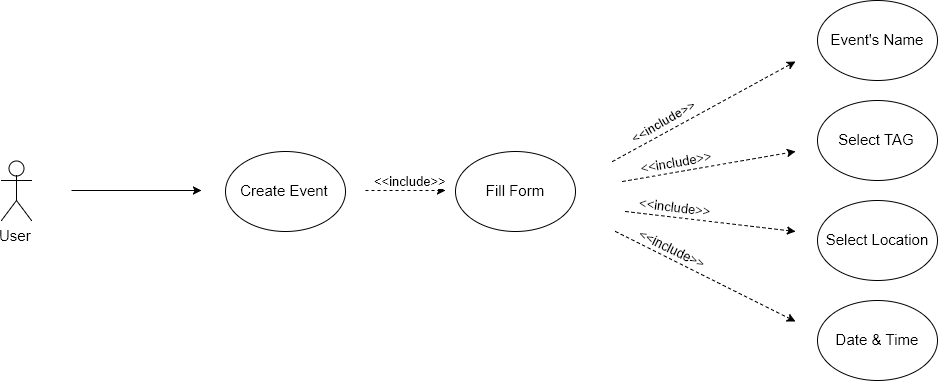
\includegraphics[scale=0.25]{Images/Use_Case/Add_Event}
	\caption{Add Event Use Case}
\end{figure}
The system will let the user add a new event to the calendar.  The user will have to set the title, date and time, carbon footprint preference and must associate the event with a TAG. 
Once done, the system will check if the event is reachable by the previous one and if there’s not overlapping. 
If the two previous conditions are confirmed, the new event will appear in the calendar.

\mysubsubsection{Give Advices About the Means of Transport}
\begin{figure}[H]
	\centering
	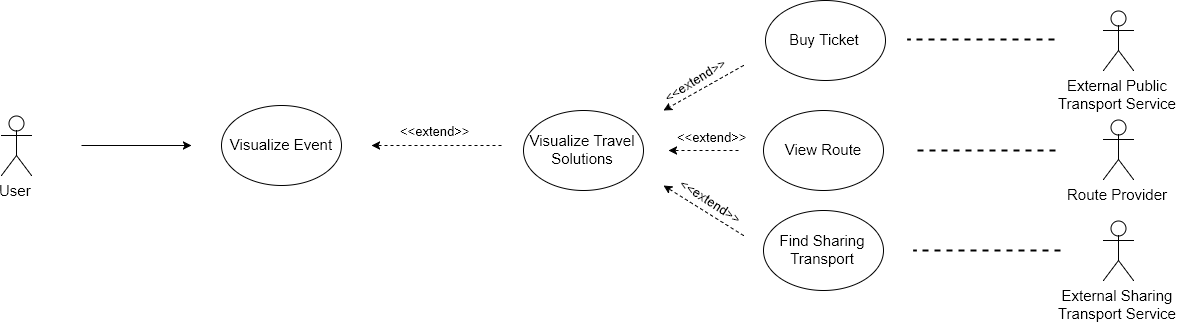
\includegraphics[scale=0.25]{Images/Use_Case/Advice_Mean}
	\caption{Advice Mean, Sharing and Ticket Purchase Use Case}
\end{figure}
The system will show the user the advices about the best means of transport for reaching every event that the he has to attend. The routes will be calculated using as starting point :
\begin{itemize}
	\setlength{\leftskip}{1cm}
	\item the previous event as the default option.
	\item the home address/outdoor accommodation if the event to reach is the first one of the day.
	\item the user position.
\end{itemize}\par
In any case, it will be possible to show the directions of every event using as starting point his position, just tapping on a specific button in the map interface.\par
The advices will follow the user’s preferences described in the TAG related to the event, keeping into account also the weather conditions and giving him warnings in the presence of strikes. Moreover, it will be given a warning when the user needs to leave in order to reach the event on time.\par
The system will also localize and show the position of the nearest car and bike sharing services.

\mysubsubsection{The Local Transport Tickets : Recommendation and Purchasing}
The system will recommend and allow to buy the best transport ticket. This feature is available just in the towns reported in the previous section.\par
Furthermore, during the trip management, after having inserted the accommodation address and the duration, the system will give back the user the tickets available, their prices and the best option that covers the entire period. The user will be able to purchase them after being addressed to the local service website/application. 

\mysubsubsection{Trip Management}
\begin{figure}[H]
	\centering
	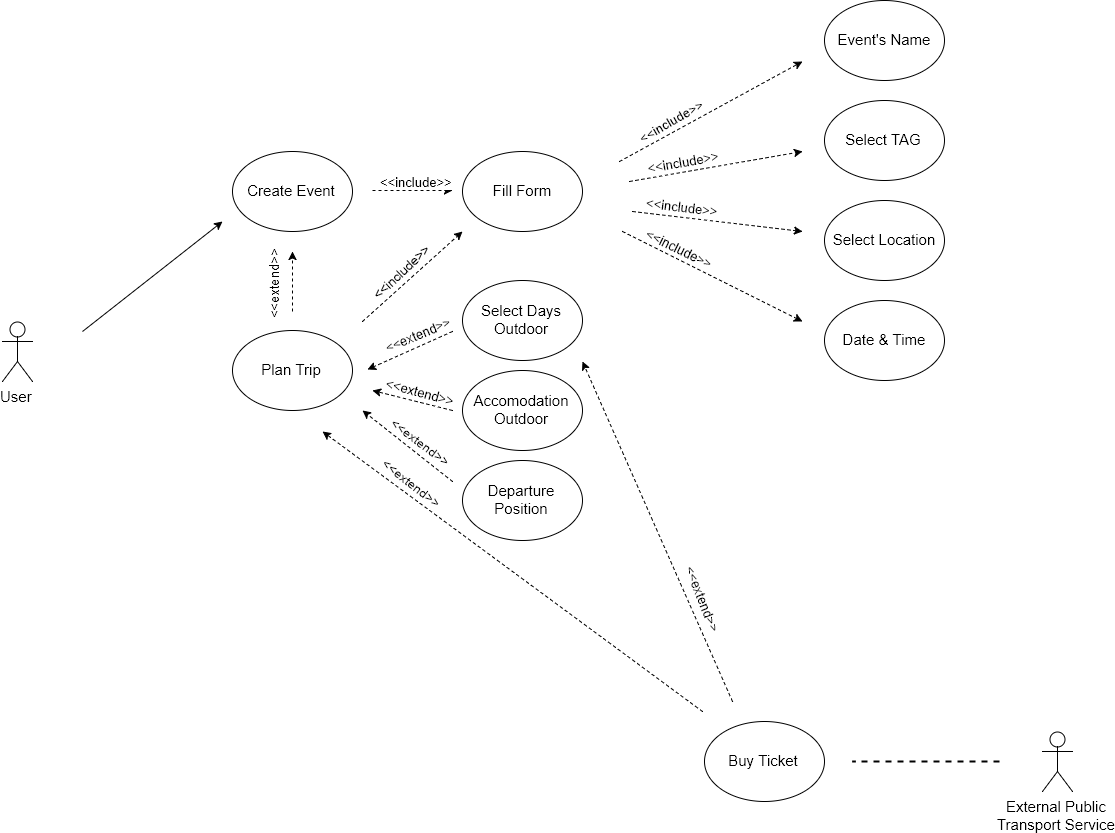
\includegraphics[scale=0.25]{Images/Use_Case/Trip}
	\caption{Trip Management and Ticket Purchase Use Case}
\end{figure}
The system will allow the user to manage trips and, by defining the accommodation and the duration, it will suggest the tickets available for reaching the desired town. It will be possible to arrange a trip directly from the calendar section. Furthermore, when an event is crated and it’s located in a town different from the user’s position, the trip’s arrangement will be prompted.\par
The travel will be represented as a special event in the calendar’s section that covers the entire travel time and contains all the information.
The user will be able to edit the trip information any time he wants, accessing the trips section.

\mysubsection{User Characteristics}
The system is suitable for any kind of user. In fact, the Travlendar+ goals are appropriate for any person who needs help for taking on the everyday organization.\\
\par
\emph{\textbf{Actors}}
\begin{itemize}
	\setlength{\leftskip}{1cm}
	\item \emph{\textbf{User : }}is a person who has done the subscription in the system. Every user, after the login process, is able to use all the system’s functionalities.

	\item \emph{\textbf{System Manager Team : }}it’s a group of engineers and programmers to whom the founders have entrusted the maintenance of the system and its upgrade for answering promptly to the users’ needs.

	\item \emph{\textbf{Client Service : }}it is a small team that has the aim of receiving and resolving users’ complaints and requests.
\end{itemize}

\mysubsection{Domanin Properties}
\begin{enumerate}
	\setlength{\leftskip}{1cm}
	\item User id must be unique.
	\item GPS position is always correct.
	\item GPS cannot be switched off.
	\item Event creation implies the user’s participation to it.
	\item Events do not overlap with each other.
	\item Every event in the calendar is reachable from the previous one.
	\item The duration of the event in the world corresponds to the duration of the one in the calendar.
	\item Only the user can create, edit and delete the event in his calendar.
	\item Public transports respect the timetables.
	\item The means of transport suggested are actual available.
	\item Every user has one calendar.
	\item External transport services always answer to the system requests.
	\item The user has to create the event before it starts.
	\item Subways, Trams and bikes do not emit CO2.
	\item Each transport mean belongs to its transport service.
	\item User can be just in one position at a time.
	\item The weather forecasts are always reliable.
	\item External services answer to the system request in no more than 5 seconds.
	\item The user who asks to purchase a ticket on the system, will actually buy the ticket in the  transport system external service.
	\item The user has to follow at least one of the warnings sent from the system.
	\item Means of transport are composed by: buses, subways, trams and trains.
\end{enumerate}